There were a number of complications when doing this project. This chapter aims 
to give some insight into what they were and how I solved them (or at least 
tried to).

\section{Power models and stats}
After getting gem5 to build and trying to learn how to set it up and use it, 
both through the ``Learning gem5'' book \cite{lowe-power_learning_2019} and by 
looking over the configuration scripts themselves, I decided to try to get the 
power models working, as power consumption was one of the main interest of the 
project. Whenever the provided \texttt{fs\_power.py} would be used as the 
configuration script, the simulator would crash right before starting the 
simulation, with the error message:
\begin{lstlisting}[basicstyle=\sffamily\footnotesize]
fatal: statistic '' (160) was not properly initialized by a regStats() function
\end{lstlisting}

I initially tried looking through documentation for both the ``Power and Thermal
Model'' \cite{noauthor_gem5_nodate-1} and the ``Stats package'' 
\cite{noauthor_gem5_nodate-3}. However, neither parts seemed to contain any 
hints as to what might be causing the crash. I also tried looking through the 
source code for the CPUs and the stats framework, but due to its scale (around 
13000 lines of code) and a lot of the code being C++ which I was not familiar 
with, this also did not solve or identify the problem.

On the 7\textsuperscript{th} of February, I raised an issue on the gem5 Jira 
pointing out that the script seemed to be broken \cite{hansen_gem5-319_2020} and
continued to look into DVFS, scheduling, and AMPs whilst waiting for a reply. My
supervisor also tried to get the script working. Just over a month later, some
of the gem5 developers got back. It turned out that they had been completely 
refactoring the way stats were done and registered, and as a result, certain 
simulated components were broken when trying to use features that relied on 
accessing the stats framework whilst a simulation was running, e.g. any 
subclass of the \texttt{MathExprPowerModel}. With one of the developers now 
being aware of the problem, an initial patch was provided within a day. After 
applying the patch and rebuilding gem5, the script managed to get past the 
initialisation step, but now crashed with the error:
\begin{lstlisting}[basicstyle=\sffamily\footnotesize]
warn: Failed to find stat 'dcache.overall_misses'
fatal: Failed to evaluate power expressions:
voltage * (2 * ipc + 3 * 0.000000001 * dcache.overall_misses / sim_seconds)
\end{lstlisting}
Based on the previous issue with registering stats, I assumed it might have been
something to do with not registering the stats the power expression was using, 
however, it turned out to be an additional bug due to the recent shift in the 
way gem5 was handling stats internally and a further patch was provided within 
a couple of days of getting back with the new error. With both patches applied, 
the \texttt{fs\_power.py} script ran without problems.

\section{Documentation and power models}
After importing the power models generated by 
\cite{walker_mattw200gemstone-applypower_2018} and setting up the scripts as
detailed in Section \ref{subsec:ext-power-mods}, the majority of the stats 
being used in the more detailed power models were unable to be found by the 
simulator. This was somewhat perplexing as the exact strings used in the 
power expressions were present in the \texttt{stats.txt} output when a 
simulation was run without the power models enabled. Trying once more to 
look through the power \cite{noauthor_gem5_nodate-1} and stats 
\cite{noauthor_gem5_nodate-3} documentation did not lead anywhere since the 
documentation does not detail which stats might exist or how to correctly 
access them. Unfortunately, I had managed to time the project at the same 
time that gem5 was migrating their website to a new one and as such, a lot 
of the documentation was missing or not in the places one would expect to 
find it. Furthermore, it turned out that the DVFS documentation was 
officially labelled out of date \cite{noauthor_gem5_nodate} and trying to 
look through more of the documentation revealed a similar pattern. Many 
pages would have a disclaimer at their top saying that they were from the 
old website and might be outdated as a result.
\begin{figure}[H]
    \centering
    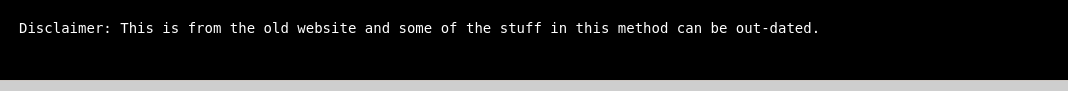
\includegraphics[width=0.9\linewidth]{screenshots/gem5-docs-disclaimer.png}
    \caption{Disclaimer initially found on many documentation pages due to 
             their recent migration from the old website}
\end{figure}

Looking at the \texttt{MathExprPowerModel} source code (Figure 
\ref{fig:relative-stat-paths}) suggested that the stat names used possibly 
had to be relative to the simulated object that was referencing them. This 
led me to try to print the output of the \texttt{getStatGroups} and 
\texttt{getStats} functions which were associated with each 
\texttt{SimObject}. The results of this can be seen in Appendix 
\ref{ch:power-model-eldritch}. However, this just seemed to confirm that 
the stats the simulator was crashing on \textit{were} present. Trying to 
specify `relative' stats, e.g. replacing the use of
\\
\texttt{system.bigCluster.clk\_domain.clock}
\\
with \texttt{clk\_domain.clock} or \texttt{Parent.clk\_domain.clock} (both 
of which seemed sensible based on the outputs from the \texttt{getStats} and
\texttt{getStatGroups} functions), did not solve the problem and still 
caused the simulator to crash, now specifying the renamed attempts as the 
stats not being found. As it was unclear which objects could be assigned a 
power model, and given that the expressions generated by 
\cite{walker_mattw200gemstone-applypower_2018} seemed to specify the full 
`path', I decided to try assigning the power models to the top-level 
\texttt{system} object and I also tried to assign power models to the 
clusters. Neither solved the problem: assigning the power model to the 
system caused the simulator to error in a different way, and assigning them 
to the clusters caused it to segfault.
\begin{figure}
    \centering
    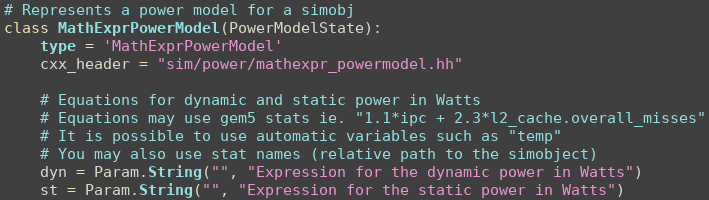
\includegraphics[width=0.9\linewidth]{screenshots/power-model-eldritchness/MathExprPowerModel-RelativeStatPath.png}
    \caption{A comment in the source code mentions that stats may have to 
             be relative to the \texttt{SimObject} they are being used with}
    \label{fig:relative-stat-paths}
\end{figure}

My next idea was that this might have something to do with the new stats 
framework and the \texttt{regStats} function which had been the source of 
previous problems. However, as far as I was able to tell, there is no 
documentation of what stats are registered by the various objects. In order 
to find this out, one has to find the \texttt{regStats} function in the C++ 
source code relevant to the \texttt{SimObject} in question. Furthermore, 
some knowledge of the object hierarchy is required as stats registered in a 
superclass are available to the power models in a subclass. One of the stats
that was not mentioned in the gem5 crash messages was the \texttt{numCycles}
stat. This stat is registered by the \texttt{BaseCpu} class and was
referable exactly as registered: by the \texttt{numCycles} string. Once I
found the source code for the voltage and clock domains (located in 
\texttt{gem5/src/sim/power/}) I discovered that they \textit{did} seem to 
register the stats that the simulator claimed to be unable to find.
\begin{figure}[H]
    \centering
    \begin{subfigure}[b]{0.45\textwidth}
        \centering
        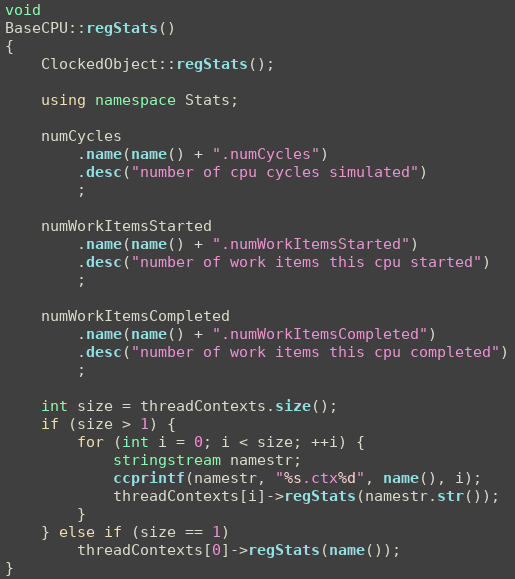
\includegraphics[width=\textwidth]{screenshots/have-to-search-src-for-regStats/base-cpu-cc-regStats.png}
        \caption{Stats registered by \texttt{BaseCpu}}
    \end{subfigure}
    \hfil
    \begin{minipage}[b]{0.45\textwidth}
        \begin{subfigure}[b]{\linewidth}
            \centering
            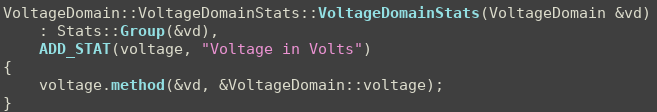
\includegraphics[width=\textwidth]{screenshots/have-to-search-src-for-regStats/voltage-domain-registers-a-stat.png}
            \caption{Stats registered by \texttt{VoltageDomain}}
        \end{subfigure}
        \\[\baselineskip]
        \begin{subfigure}[b]{\linewidth}
            \centering
            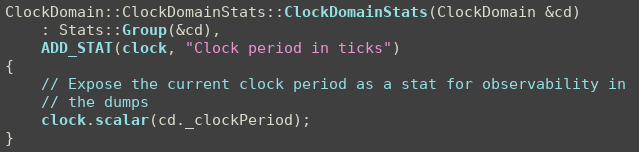
\includegraphics[width=\textwidth]{screenshots/have-to-search-src-for-regStats/clock-domain-registers-a-stat.png}
            \caption{Stats registered by \texttt{ClockDomain}}
            \label{subfig:clk-dom-regStats}
        \end{subfigure}
    \end{minipage}
    \caption{Various \texttt{regStats} functions searched to find stat 
             names}
    \label{fig:regstats-search}
\end{figure}

Having exhausted every attempt at finding and fixing what I presumed was a 
simple issue, I opened another issue on the gem5 Jira 
\cite{hansen_gem5-463_2020}. As this was now very close to the project 
deadline, I reverted back to using the toy power models because whilst not 
hardware-validated, they did produce power output which varied depending on 
the workload and DVFS state of the system, and getting some results was a 
very high priority. I also looked into potentially using a completely 
different simulator, in order to get any results. As I did not expect to 
get an answer immediately or to necessarily have the developers be able to 
solve it in an instant, I set up the experiments described in Chapter 
\ref{ch:experiments} as soon as possible.

I received a response to the issue the next day along with a pointer to 
some existing patches which could be possible solutions. However, these had 
merge conflicts with the previous patches that were applied to fix the 
\texttt{regStats} bug and eventually, by discussing the issue with the 
developer helping me, we found out that it was not a problem with the 
simulator but with the naming of the stats. The stat that the power 
expression was trying to reference was \texttt{clk\_domain.clock}. Based on 
both the \texttt{stats.txt} output and the clock domain's \texttt{regStats} 
function, this seemed to be the name of the stat. Instead, it turns out 
that the current clock value can be is accessed through the string 
\texttt{clock\_period}. This parameter only appears internally in the 
\texttt{clock\_domain.cc} file, where it is assigned to the 
\texttt{\_clockPeriod} field (see Figure \ref{fig:clock-period-src}), which 
is then used in the \texttt{regStats} method (see Figure 
\ref{subfig:clk-dom-regStats}). Other than this, there is no indication 
anywhere that this might be the stat name. Unfortunately, as I was busy 
trying to get any results ready and refactoring all the power equations 
would have taken some time, this solution never made it into the project.
\begin{figure}[H]
    \centering
    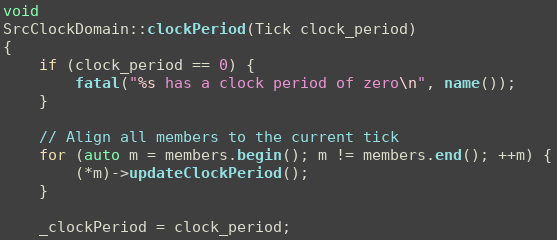
\includegraphics[width=0.85\textwidth]{screenshots/power-model-eldritchness/clock-period-src.png}
    \caption{Only uses of the \texttt{\_clockPeriod} field}
    \label{fig:clock-period-src}
\end{figure}

\section{Trying to use a different simulator}
Having seemingly exhausted most options for getting power output from gem5, my 
supervisor suggested that we try using the Sniper Simulator 
\cite{carlson_sniper_2011,carlson_evaluation_2014} due to its claims of having 
``[f]ull DVFS support'' \cite{noauthor_sniper_2020}. Sniper is only for x86 
simulation and not ARM, but it could still have been useful. Unfortunately, it 
was impossible to get it to build. Version 7.2 failed to build despite trying 
different versions of the Intel PIN tool that it depends on 
\cite{noauthor_getting_2019} and looking at the Google Groups error reporting, 
it seemed this was a common problem, even with the Docker image 
\cite{noauthor_error_2020}. Because of this, and because the toy power models in
gem5 seemed to work, no further attempts to get Sniper working were made.
